%%%%%%%%%%%%%%%%%%%%%%%%%%%%%%%%%%%%%%%%%%%%%%%%%%%%%%%%%%%%%%%%%%%%%%%%%%%%%%%%%%%%%%%%%%%%%%%%
%%%%%%%%%%%%%%%%%%%%%%%%%%%%%%%%%%%%%%%%%%%%%%%%%%%%%%%%%%%%%%%%%%%%%%%%%%%%%%%%%%%%%%%%%%%%%%%%
%%%%%%%%%%%%%%%%%%%%%%%%%%%%%%%%%%%%%%%%%%%%%%%%%%%%%%%%%%%%%%%%%%%%%%%%%%%%%%%%%%%%%%%%%%%%%%%%
%%%%%%%%%%%%%%%%%%%%%%%%%%%%%%%%%%%%%%%%%%%%%%%%%%%%%%%%%%%%%%%%%%%%%%%%%%%%%%%%%%%%%%%%%%%%%%%%
%%%%%%%%%%%%%%%%%%%%%%%%%%%%%%%%%%%%%%%%%%%%%%%%%%%%%%%%%%%%%%%%%%%%%%%%%%%%%%%%%%%%%%%%%%%%%%%%
%%%%%%%%%%%%%%%%%%%%%%%%%%%%%%%%%%%%%%%%%%%%%%%%%%%%%%%%%%%%%%%%%%%%%%%%%%%%%%%%%%%%%%%%%%%%%%%%
%%%%%%%%%%%%%%%%%%%%%%%%%%%%%%%%%%%%%%%%%%%%%%%%%%%%%%%%%%%%%%%%%%%%%%%%%%%%%%%%%%%%%%%%%%%%%%%%
%%%%%%%%%%%%%%%%%%%%%%%%%%%%%%%%%%%%%%%%%%%%%%%%%%%%%%%%%%%%%%%%%%%%%%%%%%%%%%%%%%%%%%%%%%%%%%%%
%%%%%%%%%%%%%%%%%%%%%%%%%%%%%%%%%%%%%%%%%%%%%%%%%%%%%%%%%%%%%%%%%%%%%%%%%%%%%%%%%%%%%%%%%%%%%%%%
%%%%%%%%%%%%%%%%%%%%%%%%%%%%%%%%%%%%%%%%%%%%%%%%%%%%%%%%%%%%%%%%%%%%%%%%%%%%%%%%%%%%%%%%%%%%%%%%
%%%%%%%%%%%%%%%%%%%%%%%%%%%%%%%%%%%%%%%%%%%%%%%%%%%%%%%%%%%%%%%%%%%%%%%%%%%%%%%%%%%%%%%%%%%%%%%%
%%%%%%%%%%%%%%%%%%%%%%%%%%%%%%%%%%%%%%%%%%%%%%%%%%%%%%%%%%%%%%%%%%%%%%%%%%%%%%%%%%%%%%%%%%%%%%%%
%%%%%%%%%%%%%%%%%%%%%%%%%%%%%%%%%%%%%%%%%%%%%%%%%%%%%%%%%%%%%%%%%%%%%%%%%%%%%%%%%%%%%%%%%%%%%%%%
%%%%%%%%%%%%%%%%%%%%%%%%%%%%%%%%%%%%%%%%%%%%%%%%%%%%%%%%%%%%%%%%%%%%%%%%%%%%%%%%%%%%%%%%%%%%%%%%
%%%%%%%%%%%%%%%%%%%%%%%%%%%%%%%%%%%%%%%%%%%%%%%%%%%%%%%%%%%%%%%%%%%%%%%%%%%%%%%%%%%%%%%%%%%%%%%%
%%%%%%%%%%%%%%%%%%%%%%%%%%%%%%%%%%%%%%%%%%%%%%%%%%%%%%%%%%%%%%%%%%%%%%%%%%%%%%%%%%%%%%%%%%%%%%%%
%%%%%%%%%%%%%%%%%%%%%%%%%%%%%%%%%%%%%%%%%%%%%%%%%%%%%%%%%%%%%%%%%%%%%%%%%%%%%%%%%%%%%%%%%%%%%%%%
%%%%%%%%%%%%%%%%%%%%%%%%%%%%%%%%%%%%%%%%%%%%%%%%%%%%%%%%%%%%%%%%%%%%%%%%%%%%%%%%%%%%%%%%%%%%%%%%

\section{Formulario de Cálculo Integral}
Formas básicas
\begin{align}
    &\int\,du = u + c\\
    &\int a\,du = a\int\,du = au + c\\
    &\int u^n \, du = \frac{u^{n+1}}{n+1} + C \quad (n \neq -1) \\
    &\int \frac{du}{u} = \ln{\left\lvert u\right\rvert} + c\\
    &\int\left(u \pm v \right)\,dx = \int u\,dx \pm \int v\,dx\\
    &\int e^u\,du = e^u+ c\\
    &\int a^u\,du = \frac{a^u}{\ln{(a)}} + c\mid a > 0\land a\neq 1\\
\end{align}
Funciones trigonométricas
\begin{align}
    &\int\sin{(u)}\,du = -\cos{(u)} + c\\
    &\int \cos{(u)}\,du = \sin{(u)} + c\\
    &\int\tan{(u)}\,du = \ln{\left\lvert \sec{(u)}\right\rvert } + c\\
    &\int \cot{(u)}\,  du = \ln{\left\lvert \sin{(u)}  \right\rvert} + c\\
    &\int \sec{(u)}\,  du = \ln{\left\lvert \sec{(u)} + \tan{(u)} \right\rvert } + c\\
    &\int \csc{(u)}\,  du = \ln{\left\lvert \csc{(u)} - \cot{(u)} \right\rvert } + c\\
    &\int \sec {(u)} \cdot \tan{(u)}\,  du = \sec{(u)} + c\\
    &\int \csc{(u)} \cdot   \cot {(u)}\, du = - \csc{(u)} + c\\
    &\int \sec^2{(u)}\,  du = \tan{(u)} + c\\
    &\int \csc^2{(u)}\,  du = - \cot{(u)} + c\\
    &\int \sin^2(x) \, dx = \frac{x}{2} - \frac{\sin(2x)}{4} + C \\
    &\int \cos^2(x) \, dx = \frac{x}{2} + \frac{\sin(2x)}{4} + C \\
    &\int \sin^3(x) \, dx = -\frac{\cos(x)(2 + \cos^2(x))}{3} + C \\
    &\int \cos^3(x) \, dx = \frac{\sin(x)(2 + \sin^2(x))}{3} + C \\
\end{align}
Funciones racionales
\begin{align}
    &\int \frac{du}{u^2 + a^2} = \frac{1}{a} \arctan{\left(\frac{u}{a}\right)} + c\\
    &\int \frac{du}{\sqrt{a^2 - u^2}} = \arcsin{\left(\frac{u}{a}\right)} + c\\
    &\int \frac{du}{u \sqrt{u^2 - a^2}} = \frac{1}{a}\arcsin{\left(\frac{u}{a}\right)} + c\\
    &\int \frac{du}{a^2 - u^2} = \frac{1}{2a} \ln{\left\lvert \frac{u + a}{u - a}\right\rvert } + c\\
    &\int \frac{du}{u^2 - a^2} = \frac{1}{2a}\ln{\left\lvert \frac{u - a}{u + a}\right\rvert } + c\\
    &\int \frac{du}{\sqrt{u^2 \pm a^2}} = \ln{\left\lvert u + \sqrt{u^2 \pm  a^2}\right\rvert } + c\\
    &\int \sqrt{a^2 - u^2}\, du = \frac{u}{2} \sqrt{a^2 - u^2} + \frac{a^2}{2}\arcsin{\left(\frac{u}{a}\right)} + c\\
    &\int \sqrt{u^2 \pm  a^2}\, du = \frac{u}{2}\sqrt{u^2 \pm a^2} \pm \frac{a^2}{2}\ln{\left\lvert u + \sqrt{u^2 \pm a^2} \right\rvert } + c\\
\end{align}
Integrales de Funciones Exponenciales y Logarítmicas
\begin{align*}
    \int e^{ax} \, dx &= \frac{e^{ax}}{a} + C \\
    \int e^{ax + b} \, dx &= \frac{e^{ax + b}}{a} + C \\
    \int xe^{ax} \, dx &= \frac{e^{ax}}{a^2} (ax - 1) + C \\
    \int x^n e^{ax} \, dx &= \frac{e^{ax}}{a} \left( x^n - \frac{n}{a} x^{n-1} + \frac{n(n-1)}{a^2} x^{n-2} - \cdots \right) + C \\
    \int \ln(x) \, dx &= x\ln(x) - x + C \\
    \int x \ln(x) \, dx &= \frac{x^2}{2} (\ln(x) - \frac{1}{2}) + C \\
    \int (\ln(x))^2 \, dx &= x(\ln(x))^2 - 2x\ln(x) + 2x + C \\
\end{align*}
Integrales de Funciones Hiperbólicas
\begin{align*}
\int \sinh(x) \, dx &= \cosh(x) + C \\
\int \cosh(x) \, dx &= \sinh(x) + C \\
\int \tanh(x) \, dx &= \ln|\cosh(x)| + C \\
\int \coth(x) \, dx &= \ln|\sinh(x)| + C \\
\int \text{sech}(x) \, dx &= \arctan(\sinh(x)) + C \\
\int \text{csch}(x) \, dx &= \ln|\tanh(\frac{x}{2})| + C \\
\end{align*}

\textbf{Integrales Improprias}

Caso 1: Integrales con Límite Infinito
\begin{equation*}
    \int_a^\infty f(x) \, dx = \lim_{b \to \infty} \int_a^b f(x) \, dx
\end{equation*}
Caso 2: Integrales con Descontinuidad Infinita
\begin{equation*}
    \int_a^b f(x) \, dx = \lim_{c \to a^+} \int_c^b f(x) \, dx + \lim_{d \to b^-} \int_a^d f(x) \, dx
\end{equation*}
\newpage

\subsection{Integración por Sustitución Trigonométrica}

La sustitución trigonométrica es una técnica útil para resolver integrales que involucran raíces cuadradas. Aquí se presentan los tres casos principales:

\subsubsection{Caso 1:}

Para la forma \(\sqrt{a^2 - x^2}\), utilizamos la sustitución \( u= a \sin(\theta)\), \(du = a \cos(\theta) d\theta\):
\begin{equation}
    \sqrt{a^2 - u^2} = \sqrt{a^2 - a^2 \sin^2(\theta)} = a \cos(\theta)
\end{equation}

\begin{center}
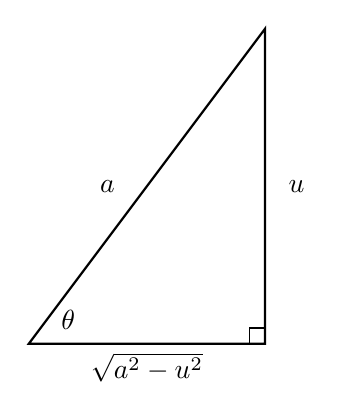
\begin{tikzpicture}
    % Triángulo rectángulo
    \draw[thick] (0,0) -- (3,0) -- (3,4) -- cycle;
    
    % Ángulo recto
    \draw (2.8,0) -- (2.8,0.2) -- (3,0.2);
    
    % Etiquetas de los lados
    \node at (1.5,-0.3) {$\sqrt{a^2 - u^2}$};
    \node at (3.4,2) {$u$};
    \node at (1.0,2) {$a$};
    
    % Etiquetas de los ángulos
    \node at (0.5,0.3) {$\theta$};
\end{tikzpicture}
\end{center}

\subsubsection{Caso 2:}

Para \(\sqrt{a^2 + x^2}\), utilizamos la sustitución \(u= a \tan(\theta)\), \(du = a \sec^2(\theta) d\theta\):
\begin{equation}
    \sqrt{a^2 + u^2} = \sqrt{a^2 + a^2 \tan^2(\theta)} = a \sec(\theta)
\end{equation}


\begin{center}
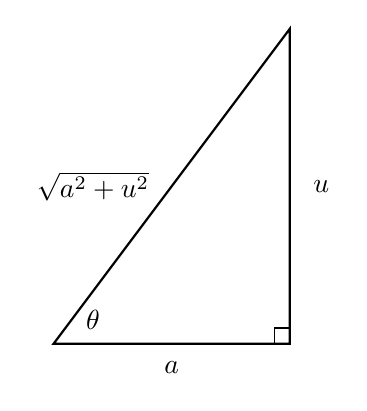
\begin{tikzpicture}
    % Triángulo rectángulo
    \draw[thick] (0,0) -- (3,0) -- (3,4) -- cycle;
    
    % Ángulo recto
    \draw (2.8,0) -- (2.8,0.2) -- (3,0.2);
    
    % Etiquetas de los lados
    \node at (1.5,-0.3) {$a$};
    \node at (3.4,2) {$u$};
    \node at (0.5,2) {$\sqrt{a^2 + u^2}$};
    
    % Etiquetas de los ángulos
    \node at (0.5,0.3) {$\theta$};
\end{tikzpicture}
\end{center}

\subsubsection{Caso 3:}

Para \(\sqrt{x^2 - a^2}\), utilizamos la sustitución \(x = a \sec(\theta)\), \(dx = a \sec(\theta) \tan(\theta) d\theta\):
\begin{equation}
    \sqrt{u^2 - a^2} = \sqrt{a^2 \sec^2(\theta) - a^2} = a \tan(\theta)
\end{equation}

\begin{center}
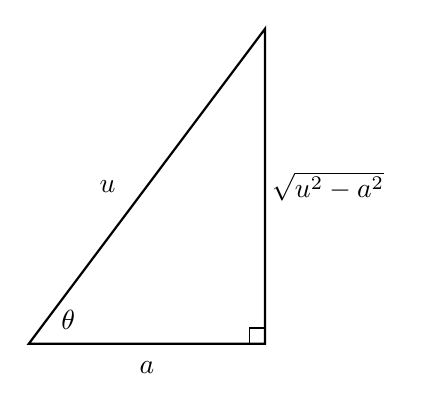
\begin{tikzpicture}
    % Triángulo rectángulo
    \draw[thick] (0,0) -- (3,0) -- (3,4) -- cycle;
    
    % Ángulo recto
    \draw (2.8,0) -- (2.8,0.2) -- (3,0.2);
    
    % Etiquetas de los lados
    \node at (1.5,-0.3) {$a$};
    \node at (3.8,2) {$\sqrt{u^2 - a^2}$};
    \node at (1.0,2) {$u$};
    
    % Etiquetas de los ángulos
    \node at (0.5,0.3) {$\theta$};
\end{tikzpicture}
\end{center}

\newpage

\subsection{Integración por Fracciones Parciales}
Es una técnica útil para integrar funciones racionales  de la forma $\frac{P(x)}{Q(x)}$ en una suma de dos o más fracciones parciales. La factorización de $Q(x)$ provee los denominadores de dichas fracciones.

\subsubsection{Caso 1: Factores Lineales Distintos}
Para una función de la forma \(\frac{P(x)}{(x-a_1)(x-a_2)\cdots(x-a_n)}\), donde \(a_1, a_2, \ldots, a_n\) son distintos:
\begin{equation}
    \frac{P(x)}{(x-a_1)(x-a_2)\cdots(x-a_n)} = \frac{A_1}{x-a_1} + \frac{A_2}{x-a_2} + \cdots + \frac{A_n}{x-a_n}
\end{equation}

\subsubsection{Caso 2: Factores Lineales Iguales}
Para una función de la forma \(\frac{P(x)}{(x-a)^n}\):
\begin{equation}
    \frac{P(x)}{(x-a)^n} = \frac{A_1}{x-a} + \frac{A_2}{(x-a)^2} + \cdots + \frac{A_n}{(x-a)^n}
\end{equation}
\subsubsection{Caso 3: Factores Cuadráticos Irreducibles Distintos}
Para una función de la forma \(\frac{P(x)}{(x^2 + b_1x + c_1)(x^2 + b_2x + c_2)\cdots(x^2 + b_nx + c_n)}\), donde los factores cuadráticos no tienen raíces reales:
\begin{equation}
    \frac{P(x)}{(x^2 + b_1x + c_1)(x^2 + b_2x + c_2)\cdots(x^2 + b_nx + c_n)} = \frac{A_1x + B_1}{x^2 + b_1x + c_1} + \frac{A_2x + B_2}{x^2 + b_2x + c_2} + \cdots + \frac{A_nx + B_n}{x^2 + b_nx + c_n}
\end{equation}
\subsection*{Caso 4: Factores Cuadráticos Irreducibles y Repetidos}
Para una función de la forma \(\frac{P(x)}{(x^2 + bx + c)^n}\):
\begin{equation}
    \frac{P(x)}{(x^2 + bx + c)^n} = \frac{A_1x + B_1}{x^2 + bx + c} + \frac{A_2x + B_2}{(x^2 + bx + c)^2} + \cdots + \frac{A_nx + B_n}{(x^2 + bx + c)^n}
\end{equation}
\newpage
